\chapter{DEAP-3600 Trigger Design $\&$ Development}
\label{chap:triggerDesign}
The trigger design serves as an integral part of the \gls{deap3} electronics system. The trigger logic is implemented on an Altera Stratix IV field programmable gate array (\gls{fpga}) which is located on the rack mounted digital trigger module (\gls{dtm}) which controls the \gls{deap3} data acquisition system (\gls{daq}). This chapter discusses the electronics system as well as the trigger design and implementation.


\section{Electronics}
The electronic architecture is divided into 3 different systems: the front end, trigger, and data acquisition as shown in Fig. \ref{Fig:OverallConcept}.

\begin{figure}[ht]
\centering
\includegraphics[height = 0.4\paperheight]{OverallConcept}
\caption{Diagram of the architecture design and data flow in the \gls{deap3} electronics system. Image credit: DEAP Collaboration.}
\label{Fig:OverallConcept}
\end{figure}

\subsection{Front End}
The front end receives a signal from each of the \gls{pmt}s through the signal conditioning boards (\gls{scb}s). The 22 primary and four veto \gls{scb}s provide several functionalities including high voltage decoupling and protection, cable termination, pulser inputs for artificial pulse injection (\gls{ppg}), an analog sum of the \gls{pmt} inputs, and a high and low gain output for each channel. The \gls{scb}s minimize the signal to noise seen by the digitizers by reshaping the signal pulses. The high gain output goes to the CAEN \gls{v1720} digitizers and its pulse width is slightly widened to allow pulses to be properly handled by the digitizer. The low gain output's pulse width is widened more than the high input and is passed to the slower CAEN \gls{v1740} digitizers. The \gls{scb} also outputs a single analog sum of its 12 \gls{pmt} inputs which is passed to the triggers digitizer board.

\subsection{Trigger}
The trigger system consists of a digital trigger module (\gls{dtm}), shown in Fig. \ref{Fig:DTM} and schematically in Fig. \ref{Fig:daqSystemCartoon}, and a pattern pulse generator (\gls{ppg}). The primary motherboard of the \gls{dtm} has three Xilinx Spartan-6 LX \gls{fpga}s which interface with three detachable daughter mezzanine boards. The mezzanine boards used in the newest \gls{dtm} arrangement are a 24-channel ADC board with three eight channel 12-bit 50 MHz ADCs; a 12-channel I/O board; and a 62.5 MHz clock board. The current \gls{dtm} configuration used outputs a master clock from this mezzanine that is daisy chained to the rest of the system. A new version, currently in the end stages of development, replaces the \gls{dtm} sourced master clock with an external master clock board as is discussed in Section \ref{sec:newClock}. The motherboard is equipped with an Altera Stratix IV GX \gls{fpga} which is used as the primary processing and communication driver for the \gls{dtm}. It is this primary \gls{fpga} that the triggering firmware is implemented on.

The \gls{dtm} receives 22 analog sums (\gls{asum}s) of 12 \gls{pmt} signals from the \gls{scb}s which are digitized by the ADC mezzanine board. The \gls{dtm} is constantly integrating the \gls{asum}s and uses \gls{fprompt} and charge to make a triggering decision. If the triggering requirements are met (as discussed in Section \ref{sec:triggerAlgorithm}) the \gls{dtm} will send a trigger command through the I/O board sending a signal to the first in a chain of digitizers which passes the trigger along to the rest in a daisy-chain arrangement.

The other main component in the trigger is the pattern pulse generator (\gls{ppg}). This board generates test signals to the \gls{scb} for self-test. Inspection of these pulses serve as a stress-test for the system and is used to test for data irregularities.
\begin{figure}[ht]
\centering
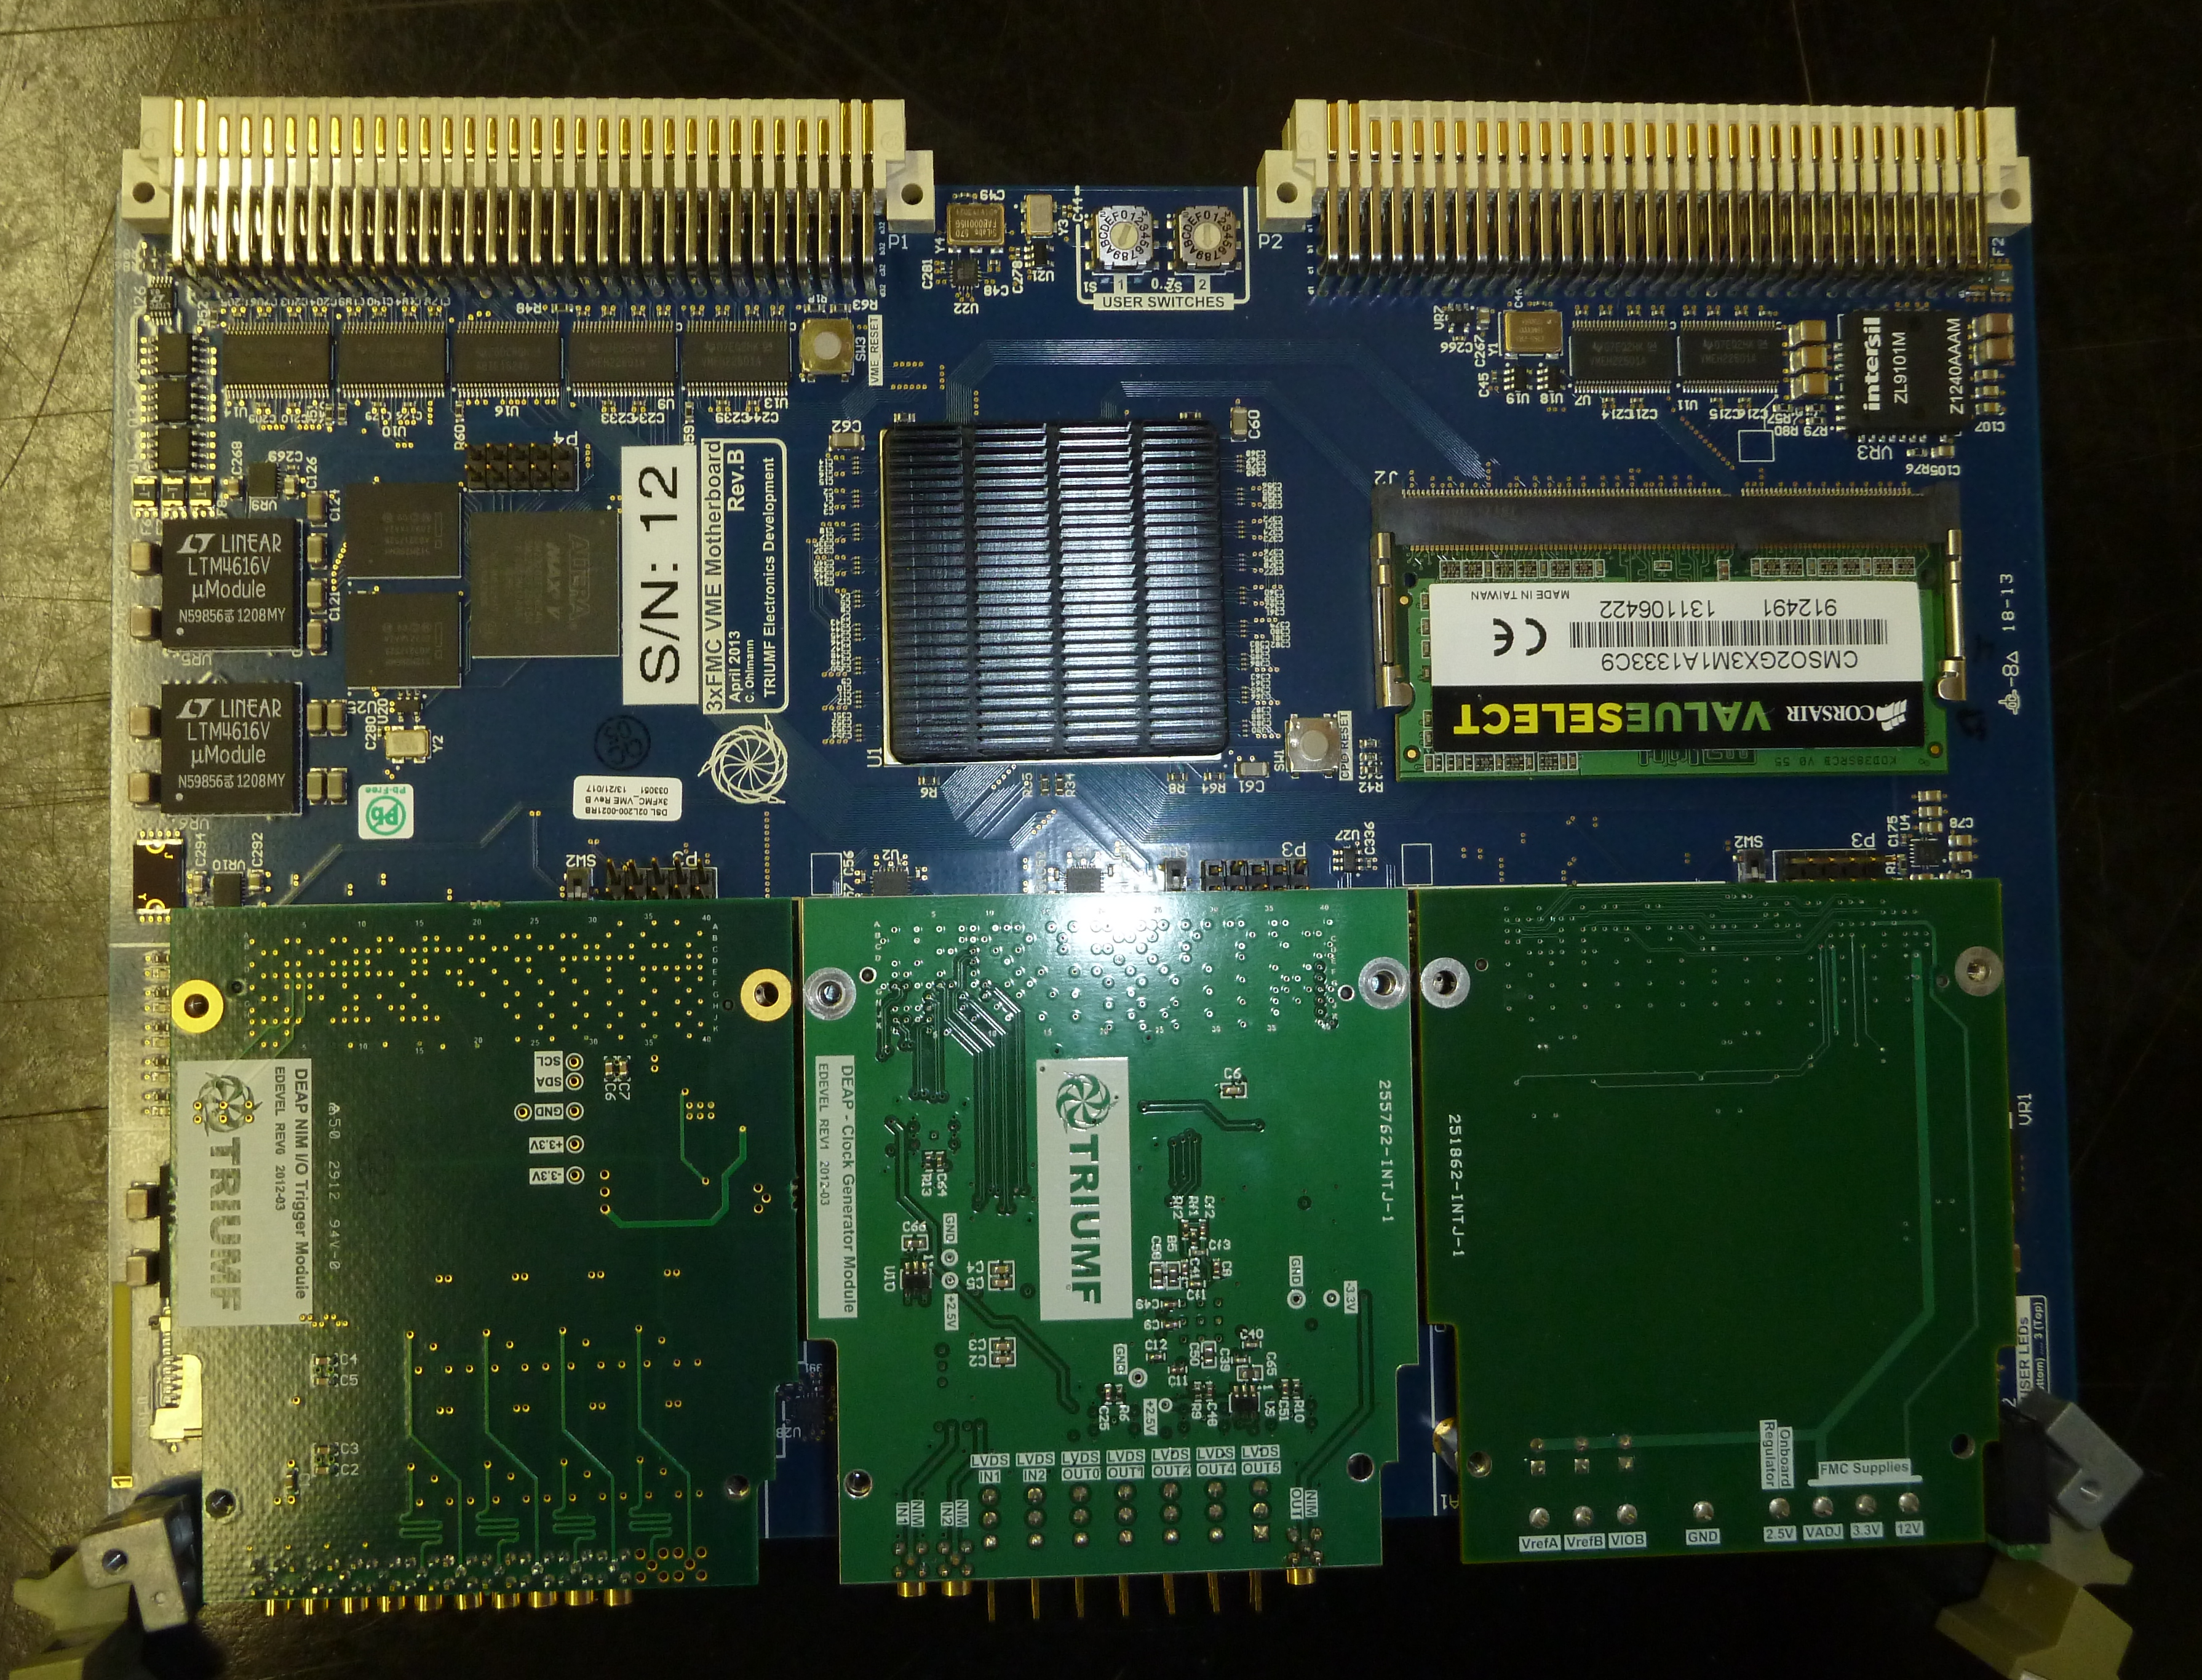
\includegraphics[height = 0.4\paperheight]{DTMModule}
\caption{The digital trigger module populated with the ADC, trigger I/O, and the clock mezzanine boards. Digital control is implemented on an Altera Stratix IV GX field programmable gate array.}
\label{Fig:DTM}
\end{figure}

\begin{figure}[ht]
\centering
\includegraphics[width = 0.85\paperwidth]{daqSystemCartoon}
\caption{Diagram of the information and signal flow in the \gls{dtm}.}
\label{Fig:daqSystemCartoon}
\end{figure}

\subsection{Data Aquisition}
The data acquisition system digitizes and saves to disk the signals from each \gls{pmt} passed from the front end \gls{scb}s. The high gain \gls{scb} signals are passed to an array of 32 CAEN \gls{v1720}s, which are eight-channel, 12-bit waveform digitizer modules that sample at 250 MS/s. The low gain signals are passed to four CAEN \gls{v1740}s which are 64-channel 12-bit waveform digitizer modules that sample at 62.5 MS/s. The slower \gls{v1740}s are used with lower gain to record any events that saturate the range of the \gls{v1720}s. The current state of the digitizers and their control is handled by logic on the Stratix IV \gls{fpga}.

\section{Trigger Algorithm}
\label{sec:triggerAlgorithm}
The \gls{fprompt} trigger analyses the 22 \gls{scb} \gls{asum} signals through the ADC mezzanine board. The signals are constantly digitized and are digitally summed together into an \gls{ass}. The firmware performs a rolling integral over a short and a long time window nominally 140 ns and 6.0 $\mu$s. The \gls{fprompt} is not explicitly calculated however it is used for event selection; for a defined \gls{fprompt} an event is recorded if

\begin{equation}
\text{E}_{\text{long}} > \text{E}_{\text{thres}} \ \& \ \text{E}_{\text{long}} >\left[ \text{E}_{\text{short}} \times \text{F}_{\text{thres}}\right].
\label{Eq:fpromptDecision} 
\end{equation}
Events are sorted using the short energy and \gls{fprompt} into one of six regions as depicted in Fig. \ref{Fig:triggerRegions}.

\begin{figure}[ht]
\centering
\includegraphics[height = 0.32\paperheight]{triggerRegions}
\caption{Trigger regions as used in the pulse shape discrimination background rejection method. Noise in the \gls{pmt}s fall under very low energy and $\beta$ events are grouped into high energy low \gls{fprompt}. The \gls{wimp} region of interest is at high \gls{fprompt} and could fall into either region of energy.}
\label{Fig:triggerRegions}
\end{figure}
The beginning of the event is taken as the first bin in the short window that maximizes the charge in that window. If the next bin in the rolling integral is lower then the last, the trigger continues to integrate forwards for a defined look ahead time (nominally 5 bins (80 ns)) to avoid local minima. If the total integrated charge does not increase past the maximum total charge within the look ahead time, then the first event bin is set as that of the maximum charge window. As the long window is integrated, a triggering signal will occur immediately a trigger condition has been meet even if the integration of the long window has not yet finished. Therefore, as multiple trigger regions (see Fig. \ref{Fig:triggerRegions}) can be passed for a single event, the final trigger type coincides with the maximum Fprompt and short window charge reached.  

Although the noise rate in the \gls{wimp} region of interest (centre one tonne fudicial volume, energy $<$ 100 keV \cite{deap3DarkMatterSearch}) is anticipated to be very low, $^{39}$Ar $\beta$-decay occurs at a high rate as shown in Table \ref{Table:backgrounds}. The \gls{fprompt} trigger uses pulse shape discrimination to mitigate (or pre-scale) $\beta$ events, reducing their recorded rate on the order of 50 times. If an event is pre-scaled the time and charge of the event is recorded, but no digitizers are triggered. To maximize sensitivity the trigger should have a low possibility of discarding events while busy, ensuring that if an event of interest occurs (\gls{wimp} or non $\beta$ background event), it will be recorded. For highest sensitivity, pre-scaling should be done only on \gls{pmt} dark noise events and $\beta$ events, so the probability of miscategorization and subsequent pre-scaling of rare events must be well understood and minimized.

In addition to the \gls{fprompt} trigger, there is a periodic trigger, an exponential random trigger which triggers the system following an exponential random variable probability distribution, and an external trigger input from the \gls{ppg}. These triggers are primarily used for diagnostic tests and calibration.



\section{Trigger Firmware Implementation}
The work done on the trigger firmware follows work done by several other \gls{deap} collaborators, notably Yair Linn and Sebastian Dittmeier at TRIUMF. This project started with an untested trigger and development here began at the debugging and testing phase.

Altera Quartus 13.0sp1 integrated development environment and the ModelSim logic simulator were used for compiling and simulation. Each change to the logic was thoroughly simulated with real waveforms from \gls{deap3} to ensure no functional regressions due to the logic. Following simulation testing, the logic is loaded onto the same hardware used in the detector. Using an arbitrary waveform generator, the trigger's functionality is confirmed. At this point the new logic release is loaded remotely onto a second \gls{dtm} at \gls{snolab}. This \gls{dtm} then replaces the currently installed \gls{dtm} to ensure that were a bug to slip by, detector time is not lost as the previous firmware can be reverted to by simply replacing the \gls{dtm} boards.

Once an operational firmware release has been installed in the detector a series of tests is run on each of the \gls{dtm} functions. Using LED light injection into the detector (see Section \ref{sec:aarfs}) triggered events are recorded along with the waveforms from the \gls{ass}s. The \gls{dtm} trigger decision is then reproduced through a C++ \gls{root} macro \cite{root} using the waveform readout (developed by Ben Smith at TRIUMF). If irregularities in the triggering decision are found, the waveform is then put through a ModelSim simulation of the trigger logic to see if the decision is reproducible or if an error has occurred.


%\FIXME{ADD DEBUGGING SECTION?}

Following this development stream, functioning \gls{fprompt} trigger logic has been installed in the \gls{deap3} detector. Chapter \ref{chap:trigStudy} discusses the study and characterization of the \gls{fprompt} trigger's behaviour and efficiency in the turn on region.


\section{Hardware Updates}
\label{sec:newClock}

Currently the clock distribution and thereby the synchronization of events for the \gls{dtm} and the \gls{v1720} and \gls{v1740} digitizers is done through a daisy chain arrangement. The master clock is generated on the \gls{dtm} at 50 MHz, a phase lock loop (\gls{pll}) raises the frequency to 100 MHz for the periodic trigger, and 62.5 MHz clock for the trigger clocking and digitizer clocks. The dedicated clock fan out mezzanine board passes the 62.5 MHz clock to the first digitizer in groups of at most six which is then passed along the chain. Each digitizer has a calculated clock phase offset to address latency in the chain as described by the manufacturer \cite{caenManual}.

The stability of this arrangement has been brought into question and therefore a new clock distribution system has been developed. The clock fan out mezzanine on the \gls{dtm} is to be replaced with a mezzanine board that receives a clock from a dedicated external master clock generator. This clock generator distributes a 62.5 MHz clock to each of the digitizers and \gls{dtm} over identical connections removing the need for an introduced clock offset. This clock arrangement should prove to be more stable, ensuring the correct synchronization of events in the \gls{daq}.

Additionally the mezzanine board that replaces the dedicated master clock fan out board on the \gls{dtm} has added functionality which allows for the direct readout of internal \gls{fpga} registers over a gigabit ethernet connection. The introduction of this system will both increase clock stability and allow for more diagnostic tests from the ethernet readout. The development of this system has recently been completed but has yet to be tested.

%is near completion but there are persistent communication issues with the front end system that have yet to be solved.
The study discussed in Chapter \ref{chap:trigStudy} uses the daisy chain clock distribution scheme and development of the new system is still on going.